\documentclass[tikz]{standalone}

\usepackage{circuitikz}
\usepackage{physics}

\usetikzlibrary{calc,positioning}

\begin{document}
	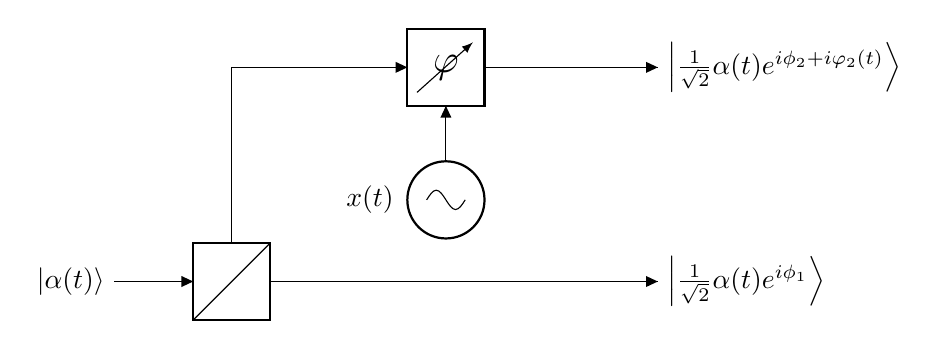
\begin{tikzpicture}
		\coordinate (in) at (0,0);
		\node (splt) [twoportsplitshape, right=of in]{};
		\node (phst) [vphaseshiftershape, above right=7em of splt] {};
		\node (osc) [vcoshape, below=2em of phst, label={180:$x(t)$}] {};
		\coordinate [right=14em of splt] (out1);
		\coordinate (out2) at (out1|-phst.west);

		\draw (in) node[left]{$\ket{\alpha(t)}$} -- (splt.west) node[inputarrow]{};
		\draw (splt.east) -- (out1) node[inputarrow]{} node[right]{$\ket{\frac{1}{\sqrt{2}}\alpha(t)e^{i\phi_1}}$};
		\draw (splt.north) -- (splt.north|-phst.west) -- (phst.west) node[inputarrow]{};
		\draw (phst.east) -- (out2) node[inputarrow]{} node[right]{$\ket{\frac{1}{\sqrt{2}}\alpha(t)e^{i\phi_2+i\varphi_2(t)}}$};		
		\draw (osc.north) -- (phst.south) node[inputarrow, rotate=90]{};
	\end{tikzpicture}
\end{document}
